\section*{Meta Activity: POGIL Research 1}

\textit{Process-Oriented Guided Inquiry Learning} (see \href{https://pogil.org/}{pogil.org}) is a student-centered, group-learning instructional strategy and philosophy developed through research on how students learn best.
The following figure is from a peer-reviewed research article about POGIL:

\begin{center}
% image from Chapter 8 of http://dx.doi.org/10.7936/K7PN93HC
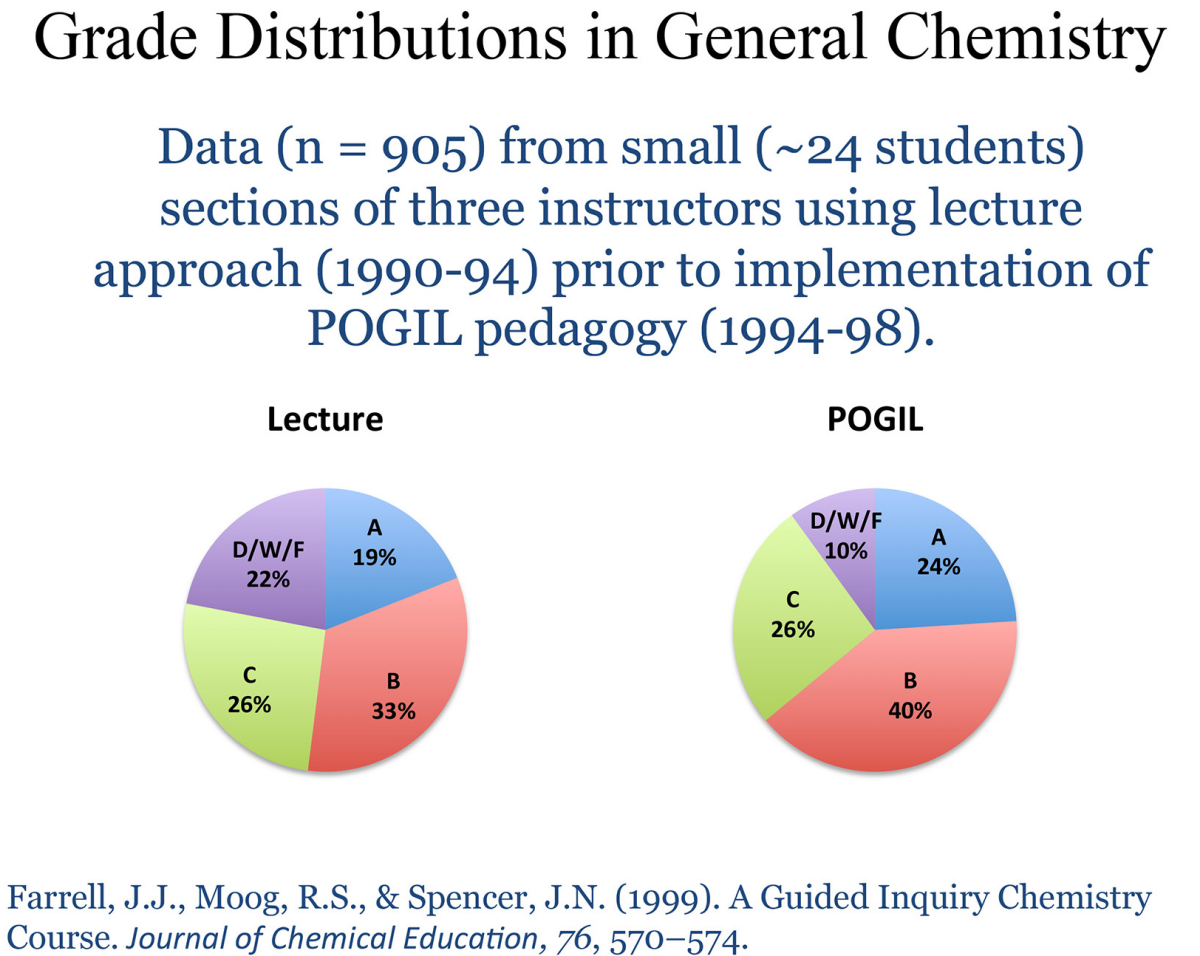
\includegraphics[width=0.60\linewidth]{pogil-grades.png}
\end{center}


\quest{7.5 min}


\Q Based on the figure above:

\begin{enumerate}
\item How many years were considered? \ans[2em]{8}
\item How many instructors were involved? \ans[2em]{3}
\item How many students were involved? \ans[2em]{905}
\end{enumerate}
\vspace{-1em}


\Q Which grade categories improved after the instructors switched to POGIL?

\begin{answer}
D/W/F decreased from 22\% to 10\%. This result is arguably the most important.
B's increased from 33\% to 40\%, and A's increased from 19\% to 24\%.
In other words, more students passed, and most students' grades increased.
\end{answer}


\Q What does the research suggest about POGIL's impact on student success?

\begin{answer}[5em]
``Students in courses employing a POGIL instructional strategy achieved a significantly higher success rate (defined as receiving an A, B, or C in the course, as compared to a D, F or withdrawal) than students who had been taught by the same instructors in previous years using a more traditional lecture-oriented approach.'' (Moog 2014)
\end{answer}
